\chapter{Theorie}
\label{cha:Theorie}

\section{Funktionsweise eines Lasers}

Ein Laser (light amplification of stimulated emission of radiation) ist eine gute Quelle für monochromatische kohärente 
elektromagnetische Wellen. Erzeugt werden diese Wellen durch die Anregung eines Lasermediums und die darauffolgende Emission
von Photonen. Angeregt wird das Medium durch eine Pumpquelle, wodurch eine Besetzungsinversion erzwungen wird.\\
Bei der Photonenemission kann zwischen zwei grundlegenden Arten unterschieden werden - eine spontane und eine stimulierte
Emission. Eine spontane Emission der 
Photonen entsteht, wenn ein Atom des angeregten Mediums aus dem energetisch erhöhten Zustand in einen niedrigeren (z.B Grundzustand) zurückfällt und 
ein Photon mit der Energie des Übergangs emittiert. 
Eine weitere Möglichkeit aus den angeregten Zuständen Photonen zu erzeugen, besteht in der stimulierten Emission. Hier wird
das Lasermedium mit Photonen bestrahlt, welche dieselbe Energie aufweisen, wie die Differenz der zwei Energiezustände. Dadurch werden Photonen emittiert,
welche dieselben Charakteristika (Ausbreitungsrichtung, Energie, Phase und Polarisation) wie die, die zur Emission angeregt haben besitzen. Das zur Emission verwendete
Photon wird hierbei nicht absorbiert. Die spontane und stimulierte 
Emission sind schematisch in \autoref{fig:emission} dargestellt.
\begin{figure}
    \centering
    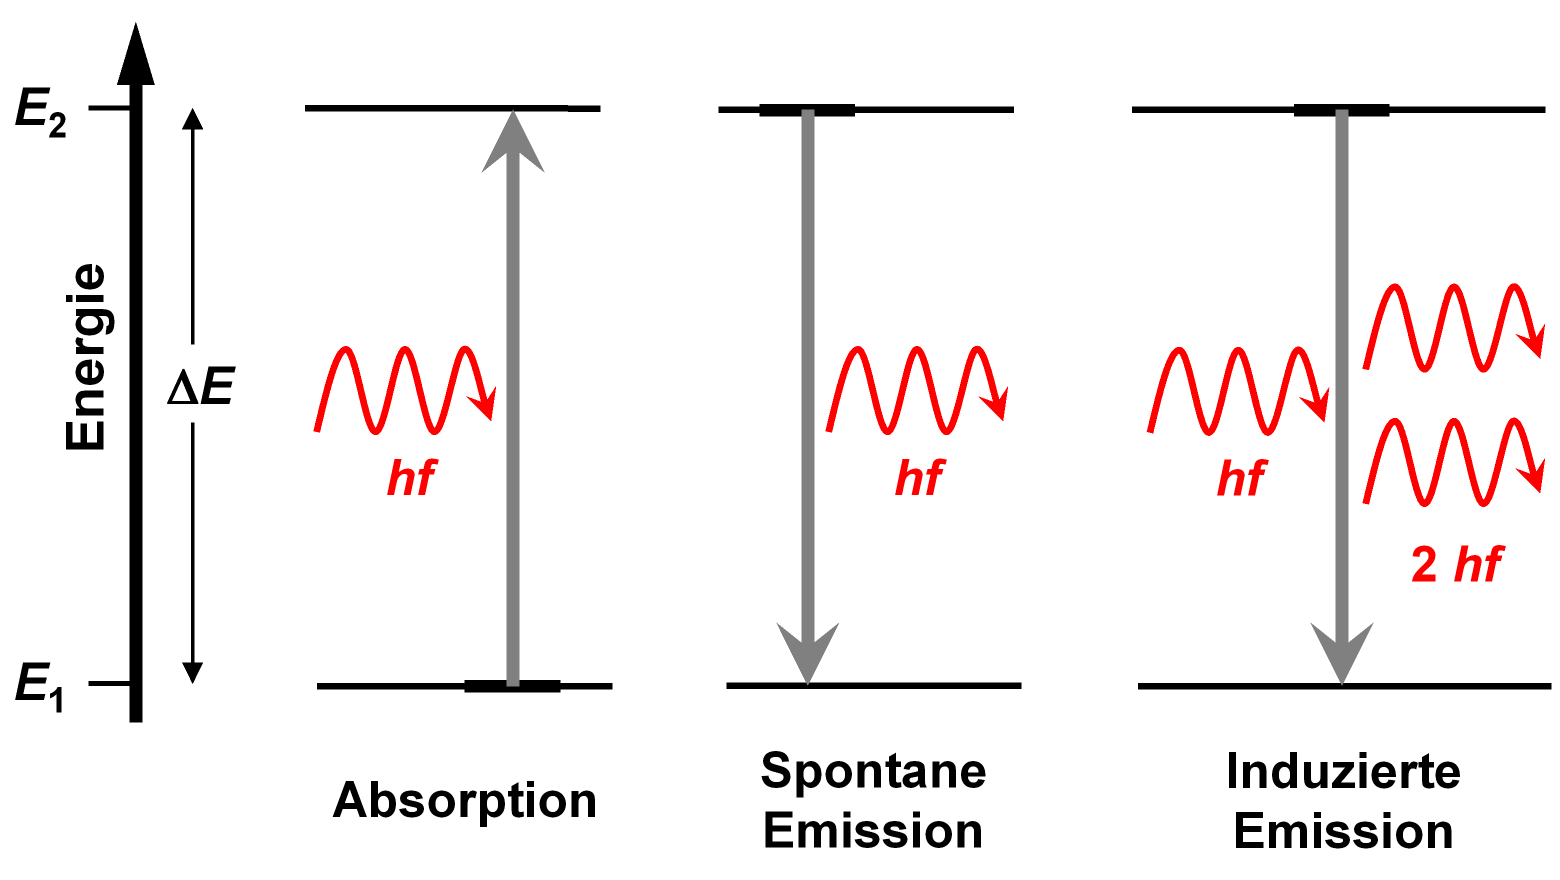
\includegraphics[width = \textwidth]{v61_bilder/emission.png}
    \caption{Schematische Darstellung der spontanen Emission (Mitte) und der stimulierten Emission (Rechts) \cite{Emission}.}
    \label{fig:emission}
\end{figure}
\\Bei einem Laser werden diese emittierten Photonen auch gleichzeitig zur stimulierten Emission weiterer Photonen verwendet. Hierdurch
entsteht ein Selbstverstärkender Effekt. Damit das entstehende elektromagnetische Feld wieder auf das Lasermedium trifft, wird ein Resonator verwendet.

\section{Der He-Ne Laser}

Der hier verwendete Lasers beinhaltet ein He-Ne Gasgemisch. Das Verhältnis der Atome beträgt etwa 5:1. Pro
Neonatom sind dementsprechend etwa 5 Heliumatome vorhanden. Die charakteristischen Eigenschaften des Lasers entstehen hier ausschließlich
durch die Neonatome. Das Helium dient als Pumpgas. Die He-Atome werden stetig durch elektrische Entladung im Laserrohr angeregt. Hierfür wird ein starker elektrischer Strom angelegt.
Das Rohr steht unter einem niedrigen Druck von $p = \qty{1}{\mathrm{Torr}}$\cite{v61}.\\
Die Pumpquelle ist notwendig, um eine Besetzungsinversion des Neongases hervorzurufen. Es sollen sich also mehr Atome in einem angeregten
Zustand befinden, als im Grundzustand. Im thermischen Gleichgewicht ist dies nicht der Fall. Ohne eine solche Besetzungsinversion ist die Wahrscheinlichkeit, dass ein vorher emittiertes
Photon lediglich wieder absorbiert wird höher, als die Wahrscheinlichkeit, dass dieses eine stimulierte Emission auslöst. Die stimulierte
Emission muss allerdings stattfinden, damit ein selbstverstärkender Effekt des Lasers auftreten kann.
Diese Besetzungsinversion wird dadurch realisiert, dass die angeregten He-Atome ihre Energie durch elastische Stöße mit Neonatomen übertragen,
wodurch diese wiederum in einen energetisch höheren Zustand gebracht werden. \\
Die Neonatome werden primär in zwei Zustände angeregt. Einerseits der 5s-Zustand und andererseits der 4s-Zustand. Diese angeregten
Zustände fallen entweder in den 4p- (nur für 5s) oder den 3p-Zustand hinab. Zu beobachten sind somit 3 spezifische Energien der Photonen.
Am intensivsten ist hier der 5s zu 3p Übergang. Der durch diesen Übergang emittierten Photonen haben eine Energie von 
$\Delta E = \qty{20.66}{\electronvolt} - \qty{18.70}{\electronvolt} = \qty{1.96}{\electronvolt}$\cite{Wikipedia_HeNe}, entsprechend einer 
Wellenlänge von $\lambda = \qty{632.8}{\nano\metre}$ und einer Frequenz von $\nu = \frac{c}{\lambda} \approx \qty{474}{\mega\hertz}$.
Die Übergänge im Heliumatom sind in \autoref{fig:helium} schematisch gezeigt.
\begin{figure}
    \centering
    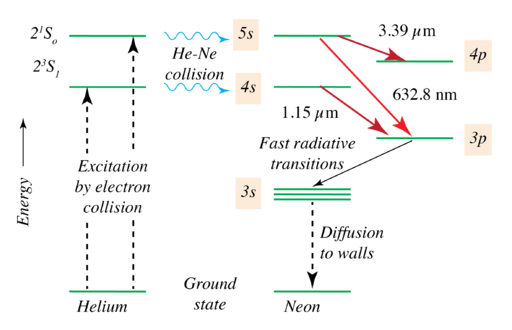
\includegraphics[width = 0.7\textwidth]{v61_bilder/helium.png}
    \caption{Schematische Darstellung der Energieübergänge des angeregten Heliumatoms\cite{Wikipedia_HeNe}.}
    \label{fig:helium}
\end{figure}
\\Da die Gas Atome sich innerhalb des Laserrohrs mit einer bestimmten mittleren Geschwindigkeit bewegen, kommt es durch den Doppler-Effekt zu leicht unterschiedlichen
Frequenzen der emittierten Photonen. Neon-Atome welche sich bei der Emission eines Photons sich in dessen Ausbreitungsrichtung bewegt hat, emittieren Photonen mit einer
leicht höheren Frequenz als solche, die sich in die entgegengesetzte Richtung bewegt haben. Diese emittieren Photonen mit einer leicht niedrigeren Frequenz. Dadurch entsteht
ein Frequenzspektrum, welches in etwa $\Delta f = \qty{1.5}{\giga\hertz}$\cite{Wikipedia_HeNe} breit ist.

\section{Resonator}
\label{sec:resonator}

Damit ein Selbstverstärkender Effekt auftreten kann, muss das entstehende elektromagnetische Feld reflektiert werden. Hierfür wird ein System aus zwei
hochreflektierenden Spiegeln verwendet, welche jeweils an den Öffnungsfenstern des Lasermediums angebracht werden. Das Lasermedium befindet sich in einem 
zylindrischen Behälter; Die Öffnungsfenster befinden sich jeweils an Boden und Deckel des Zylinders. Die verwendeten Spiegel bestehen aus einem hochreflektierenden
Spiegel mit einem Reflektionsanteil von über $\qty{99}{\%}$ und einem Auskopplungsspiegel, welcher zwischen $\qty{1.5}{}-\qty{1.8}{\%}$ der Strahlungsintensität
auskoppelt und für Untersuchungen der Lasereigenschaften bereitstellt.\\
Die verwendeten Spiegel können entweder flach ($r = \infty$) sein oder eine Wölbung aufweisen. Je nach Anordnung und Abstand der Spiegel entsteht
eine bestimmte Abschwächung der Strahlenintensität. Diese Abschwächung lässt sich über die Multiplikation der Resonatorparameter
\begin{equation}
    g_i = 1 - \frac{L}{r_i}
\end{equation}
bestimmen, wobei L der Abstand der zwei Spiegel (die Resonatorlänge) und $r_i$ der Radius des jeweiligen Spiegels ist. Die Stabilitätsbedingung ergibt sich somit zu 
\begin{equation}
    \label{eqn:stabil}
    0 \leq g_1 \cdot g_2 \leq 1.
\end{equation}
Die geringsten Verluste sind für eine Anordnung zu erwarten, bei der beide Spiegelbrennpunkte zusammenfallen. Ausschlaggebend für eine erfolgreiche Selbstverstärkung
des Lasers ist, dass die Verluste innerhalb des Resonator geringer sein müssen, als die durch stimulierte Emission erreichte Verstärkung.\\
Innerhalb des Resonators bilden sich elektromagnetische Moden, $\mathrm{TEM}_{lpq}$ genannt, aus. Diese Moden bilden sich durch eine Erfüllung der Resonanzbedingung aus.
Hierbei wird zwischen drei Modenarten unterschieden. Die Indizes $l$ und $p$ stehen jeweils für die transversalen Moden orthogonal zu der Ausbreitungsrichtung in x-
und y-Richtung. $l$ steht für die longitudinalen Moden in Ausbreitungsrichtung. Dabei bezeichnet ein Wert von $0$ die Grundmode und ein höherer Wert die höheren Moden.\\
Die Feldverteilung des elektromagnetischen Feldes orthogonal zur Ausbreitungsrichtung ist durch
\begin{equation}
    E_{lp}(x) \propto H_l(x) H_p(x) e^{\frac{-x^2}{2}}
\end{equation}
gegeben, wobei $H_i(x)$ jeweils die Hermite-Polynome der entsprechenden Transversalmoden sind. Die Intensität des Strahl orthogonal zur Ausbreitungsrichtung ist hierbei
proportional zum Betragsquadrat der Feldverteilung:
\begin{equation}
    \label{eqn:intensity}
    I_{lp}(x) \propto I_0 \lvert E_{lp}(x) \rvert ^2 \propto I_0 \lvert H_l(x) H_p(x) e^{\frac{-x^2}{2}} \rvert ^2.
\end{equation}
$I_0$ ist die maximal erreichbare Intesität in der Mitte des Strahls. Für höhere Moden werden auch höhere Hermite-Polynome verwendet, wodurch die Stärke der
Abhängigkeit in x-Richtung zunimmt. Hierdurch haben Höhere Moden allgemein stärkere Verluste. Die verlustfreiste Mode ist also die Grundmode, gegeben durch $\mathrm{TEM}_{000}$.
Das nullte Hermite-Polynom ist konstant, wodurch sich die Intensität zu
\begin{align}
    I_{00}(x) &\propto I_0 \lvert e^{-x^2} \rvert ,\\
    I_{00}(r) &\propto I_0 e^{\frac{-2r^2}{\omega^2}}
\end{align}
ergibt. Hier ist $r$ der radiale Abstand zum Strahlmittelpunkt und $\omega(z) = \omega_0\sqrt{1+(\frac{\omega_d z}{\omega_0})^2}$ der Radius des Strahls in Abhängigkeit der z-Richtung.
$\omega_0$ ist dabei der Radius bei $z=0$ und $\omega_d = \frac{\lambda\omega_0}{\pi}$ die Divergenz des Strahls.